\subsection{Étale maps}

DEFINITION 2. --- Let E and B be topological spaces, let \(p\colon\mathrm{E}\to\mathrm{B}\) be a map and let \(x\) be a point of E. One says that the map \(p\) is topologically étale at \(x\) if there exists a neighborhood U of \(x\) in E and a neighborhood V of \(p(x)\) in B such that \(p\) induces a homeomorphism from U onto V.

One says that the map p is topologically étale if it is topologically étale at every point x of E.

When there is no possible confusion (cf. Example 3 below), one says étale instead of topologically étale. Instead of saying that \(p\colon \mathrm{E}\to \mathrm{B}\) is an étale map, one also says that the B-space \((\mathrm{E},p)\) is an étale B-space, or simply that E is an étale space over B, when no doubt is possible as to the map \(p\).

Remarks. --- 1) The set of points of E at which a map \(p \colon \mathrm{E} \to \mathrm{B}\) is étale is an open subset U of E and the restriction of p to U is an étale map from U to B.

\begin{enumerate}
\def\labelenumi{\arabic{enumi})}
\setcounter{enumi}{1}
\tightlist
\item
  An étale map is continuous and open (TG, I, p. 33, prop. 5); in particular, the image of an étale map is open. Conversely, if \(p \colon \mathrm{E} \to \mathrm{B}\) is a continuous and open mapping, and if every point x of E has a neighborhood V such that the map \(p \mid \mathrm{V}\) is injective, the map p is étale. The fibers of an étale map are discrete.
\end{enumerate}

Examples. --- 1) Let B be a topological space and \((\mathrm{U}_{i})_{i\in\mathrm{I}}\) a family of subsets of B. Let E denote the sum space of the family \((\mathrm{U}_{i})_{i\in\mathrm{I}}\) and \(p: E \to B\) the map induced by the canonical injections of the \(U_{i}\) in B. For the map p to be étale, it is necessary and sufficient that the \(U_{i}\), \(i \in I\), all be open.

\begin{enumerate}
\def\labelenumi{\arabic{enumi})}
\setcounter{enumi}{1}
\item
For a holomorphic function \(f\colon U \to \mathbf{C}\) to be an étale map, it is necessary and sufficient that its derivative does not vanish.
\item
  An étale morphism of varieties (VAR, R, 5.7.8) is a topologically étale map, but there exist morphisms of real varieties that are topologically étale and are not étale morphisms. This is the case, for example, of the map \(x \mapsto x^3\) from \(\mathbf{R}\) into \(\mathbf{R}\). However, a morphism of complex analytic varieties that is topologically étale is an étale morphism (I, p. 141, exerc. 6).
\end{enumerate}

PROPOSITION 6. — Let X, Y, Z be topological spaces and let \(f\colon X\to Y\) , \(g\colon Y\to Z\) be maps.

\begin{enumerate}
\def\labelenumi{\alph{enumi})}
\item
  Suppose that f and g are étale; then \(g \circ f\) is étale.
\item
  Suppose that \(g\) is étale, \(f\) is continuous and \(g \circ f\) is open. Then \(f\) is open.
\item
  Suppose that \(g \circ f\) and \(g\) are étale and that \(f\) is continuous. The map \(f\) is then étale.
\item
  Suppose that \(g \circ f\) is étale and that the map \(f\) is continuous and open; then, \(f\) is étale and \(g\) is étale at every point of \(f(\mathrm{X})\) .
\end{enumerate}

Let us prove (a). Suppose that \(f\) and \(g\) are étale. They are then continuous and open, so the map \(g \circ f\) is continuous and open. Let \(x\) be a point of X. There exists a neighborhood W of \(f(x)\) in Y such that \(g \mid \mathrm{W}\) is injective, and a neighborhood V of \(x\) in X, contained in \(f(\mathrm{W})\), such that \(f \mid \mathrm{V}\) is injective; the map \((g \circ f) \mid \mathrm{V}\) is then injective. This proves that the map \(g \circ f\) is étale (Remark 2).

Let us prove b). Let x be a point of X and W an open neighborhood of \(f(x)\) such that g induces a homeomorphism from W onto the open set \(g(\mathrm{W})\). Let V be a neighborhood of x such that \(f(\mathrm{V})\) is contained in W; then, \(g \circ f(\mathrm{V})\) is a neighborhood of \(g \circ f(x)\), therefore \(f(\mathrm{V})\) is a neighborhood of \(f(x)\) in the open set W, and also in Y. This proves that the map f is open (TG, I, p. 33, prop. 5).

Let us prove c). By b), f is open. Let x be a point of X. Since \(g \circ f\) is étale, there exists a neighborhood V of x in X such that \(g \circ f \mid V\) is injective. Thus, \(f \mid V\) is injective and f is étale (I, p. 29, remark 2).

Let us prove d). Let \(x\) be a point of \(X\) and set \(y = f(x)\). There exists an open neighborhood \(V\) of \(x\) such that \(g \circ f\) induces a homeomorphism from \(V\) onto the open set \(g \circ f(V)\). As the map \(f\) is open, \(f(V)\) is an open neighborhood of \(y\). The map \(f|_V\colon V \to f(V)\) induced by \(f\) by passing to subspaces is continuous, open, and bijective; it is therefore a homeomorphism, so that \(f\) is étale at \(x\). Moreover, the map \(g\) induces a homeomorphism of \(f(V)\) onto \(g \circ f(V)\), hence is étale at \(y\).

COROLLARY 1. — Let B be a topological space. A B-morphism from one étale B-space to another is étale.

This follows from assertion c) of Prop. 6.

COROLLARY 2. --- Let B be a topological space; a bijective B-morphism from one étale B-space to another is a B-isomorphism.

By corollary 1, such a morphism is étale; it is therefore open (I, p. 29, remark 2). If it is bijective, it is a B-isomorphism.

COROLLARY 3. --- Let p: E → B be an étale map. Every continuous section of p induces a homeomorphism of B onto an open subset of E.

Indeed, such a section is étale (corollary 1), hence open.

COROLLARY 4. --- Let p: E → B be an étale and separated map. Suppose that E is connected and that p admits a section. Then p is a homeomorphism.

Let \(s\) be a section of \(p\) ; since \(p\) is étale, the image of \(s\) is open in E (Corollary 3); it is also closed, since \(p\) is separated (I, p. 27, prop. 3). Since E is connected, we have \(s(\mathrm{B}) = \mathrm{E}\) and \(p\) is a homeomorphism.

PROPOSITION 7. --- Let \(p\colon E \to B\) be a continuous map. For the map \(p\) to be étale, it is necessary and sufficient that it be open and that the diagonal \(\Delta_{E}\) of \(E \times_{B} E\) be open in \(E \times_{B} E\).

Suppose first that the map p is étale. Then it is open and every point of E has a neighborhood V such that \(p|V\) is injective, which amounts to saying that one has \((\mathrm{V} \times \mathrm{V}) \cap (\mathrm{E} \times_{\mathrm{B}} \mathrm{E}) \subset \Delta_{\mathrm{E}}\) . Therefore, \(\Delta_{E}\) is an open subset of \(E \times_{B} E\) .

Conversely, suppose that p is an open mapping and that \(\Delta_{\mathrm{E}}\) is an open subset of \(\mathrm{E} \times_{\mathrm{B}} \mathrm{E}\) . Let x be a point of E. Let V be an open neighborhood of x in E such that \((\mathrm{V} \times \mathrm{V}) \cap (\mathrm{E} \times_{\mathrm{B}} \mathrm{E})\) is contained in \(\Delta_{\mathrm{E}}\) . Then, \(p \mid \mathrm{V}\) is injective. By Remark 2, I, p. 29, the map p is étale.

PROPOSITION 8. --- Let

\pandocbounded{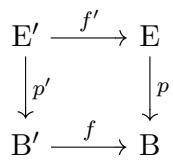
\includegraphics[keepaspectratio]{images/part001_e4ab0ebd.jpg}}

a Cartesian square. If the morphism p is étale, then the morphism p' is étale. Conversely, if the morphism p' is étale and the morphism f is universally strict and surjective, then the morphism p is étale.

Suppose that the map p is étale. In particular, it is open and \(p'\) is open (I, p. 17, prop. 8). Consider then the Cartesian square (I, p. 13, example 1)

\[
\begin{array}{c} \mathrm{E} ^ {\prime} \times_ {\mathrm{B} ^ {\prime}} \mathrm{E} ^ {\prime} \xrightarrow {\varphi} \mathrm{E} \times_ {\mathrm{B}} \mathrm{E} \\ \Biggl \downarrow q ^ {\prime} \qquad \qquad \qquad \qquad \Biggl \downarrow q \\ \mathrm{B} ^ {\prime} \xrightarrow {f} \mathrm{B}. \end{array}
\]

We have \(\Delta_{\mathrm{E}^{\prime}} = \overline{\varphi}^{1}(\Delta_{\mathrm{E}})\) (loc. cit.). Moreover, the diagonal \(\Delta_{\mathrm{E}}\) is open in \(\mathrm{E} \times_{\mathrm{B}} \mathrm{E}\) (prop. 7), hence the diagonal \(\Delta_{\mathrm{E}^{\prime}}\) is open in \(\mathrm{E}^{\prime} \times_{\mathrm{B}^{\prime}} \mathrm{E}^{\prime}\). This proves that the map \(p^{\prime}\) is étale (loc. cit.).

Suppose now that the map \(f\) is surjective and universally strict, and let the map \(p'\) be étale. Then, \(p'\) is open, therefore \(p\) is open (I, p. 21, prop. 11, \(a\)). On the other hand \(\Delta_{\mathrm{E}'}\) is an open subset of \(\mathrm{E}' \times_{\mathrm{B}'} \mathrm{E}'\). Since \(\Delta_{\mathrm{E}'} = \overline{\varphi}^{1}(\Delta_{\mathrm{E}})\) and the map \(\varphi\) is surjective and strict (I, p. 20, def. 6), \(\Delta_{\mathrm{E}}\) is open in \(\mathrm{E} \times_{\mathrm{B}} \mathrm{E}\). By prop. 7, the map p is étale.

COROLLARY. --- Let B be a topological space. The fiber product of two étale B-spaces is an étale B-space.

Let \((\mathrm{E}, p)\) and \((\mathrm{E}^{\prime}, p^{\prime})\) be étale B-spaces. The map \(pr_{1}: E \times_{B} E^{\prime} \to E\) is étale (prop. 8), hence the map \(p \circ pr_{1}: E \times_{B} E^{\prime} \to B\) is étale (prop. 6, a)).

Remark 3. --- Let

\pandocbounded{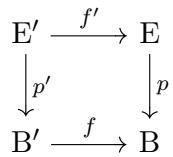
\includegraphics[keepaspectratio]{images/part001_b818a80c.jpg}}

a Cartesian square. If the map p is étale and the map f is strict, then the map \(f'\) is strict. Indeed, under these hypotheses, every point of E has an open neighborhood U such that p induces a homeomorphism from U onto the open set \(p(\mathrm{U})\) . The map \(p'\) induces then a homeomorphism of \((f')^{-1}(\mathrm{U})\) onto \(f^{-1}(p(\mathrm{U}))\). The map f induces a strict map from \(f^{-1}(p(\mathrm{U}))\) onto \(p(\mathrm{U})\) (I, p. 20) and the map \(f'\) therefore induces a strict map from \((f')^{-1}(\mathrm{U})\) into U. It follows that the map \(f'\) is strict (I, p. 23, corollary 2).

